\documentclass{article}
\usepackage[utf8]{inputenc}
\usepackage{subfig}
\usepackage{amsmath}

\usepackage{graphicx}
\usepackage[legalpaper, portrait, margin=0.5cm]{geometry}

\thispagestyle{empty}
\begin{document}

\begin{figure}[h]
        \centering
        \subfloat[horizontal cut at $y=0$]{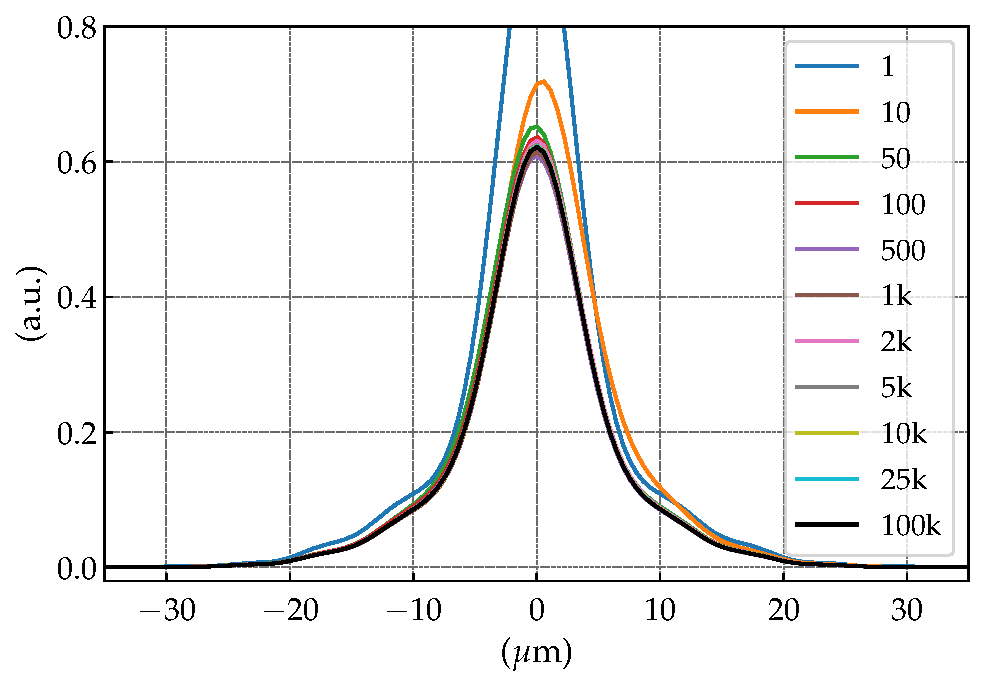
\includegraphics[height=4.5cm]{figures/id18_c01_7p0keV_x_cut.pdf}}\hspace{0.1cm}
        \subfloat[vertical cut at $x=0$]{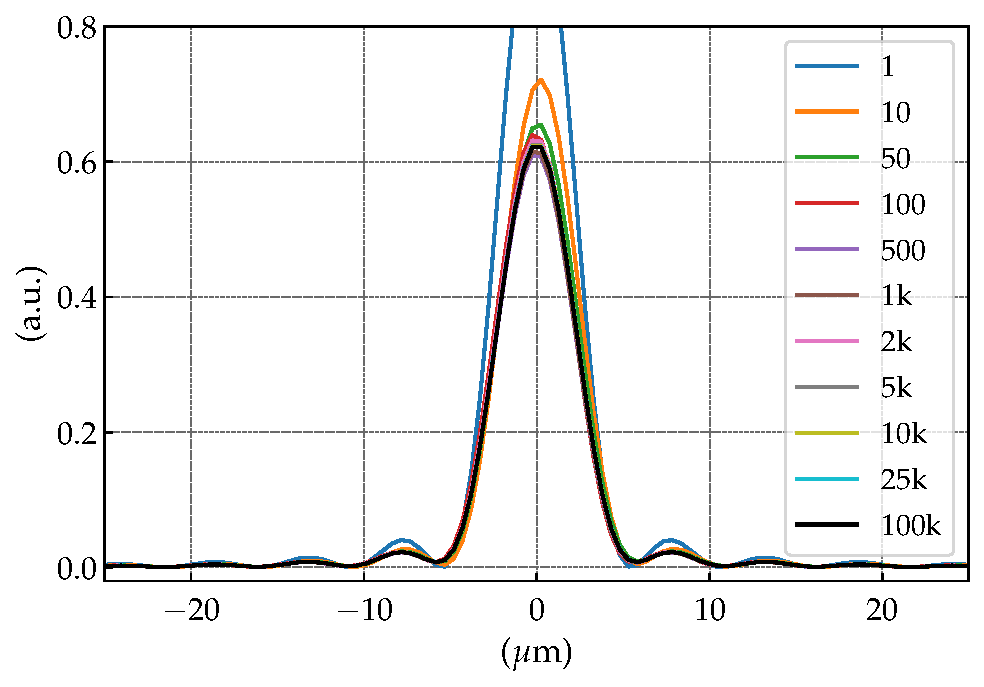
\includegraphics[height=4.5cm]{figures/id18_c01_7p0keV_y_cut.pdf}} \\
        \subfloat[relative error std. deviation]{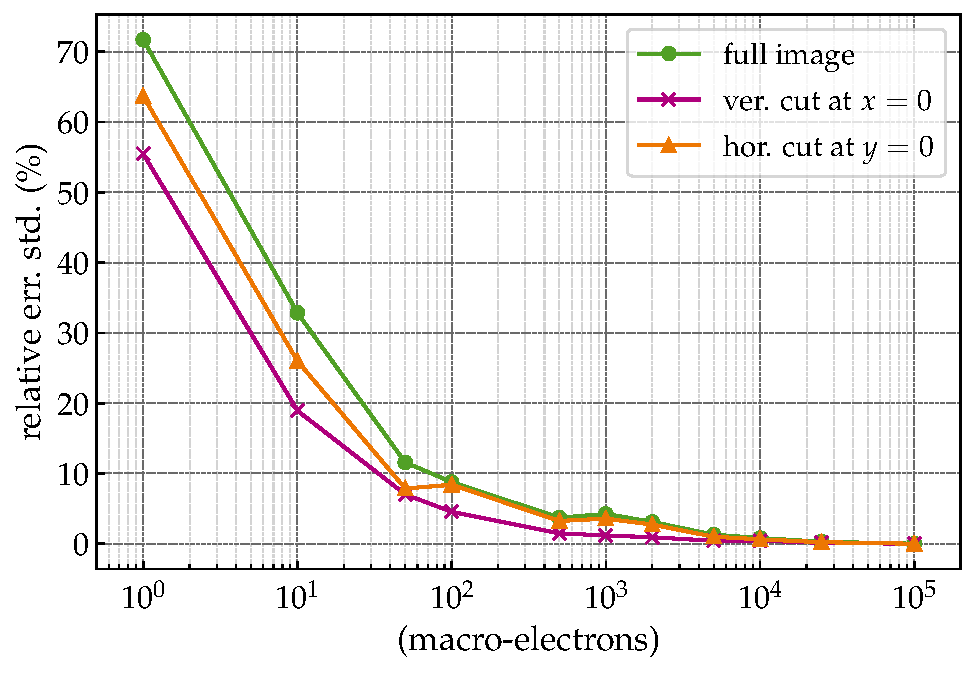
\includegraphics[height=4.5cm]{figures/id18_c01_7p0keV_errs.pdf}}\hspace{0.1cm}
        \subfloat[peak intensity]{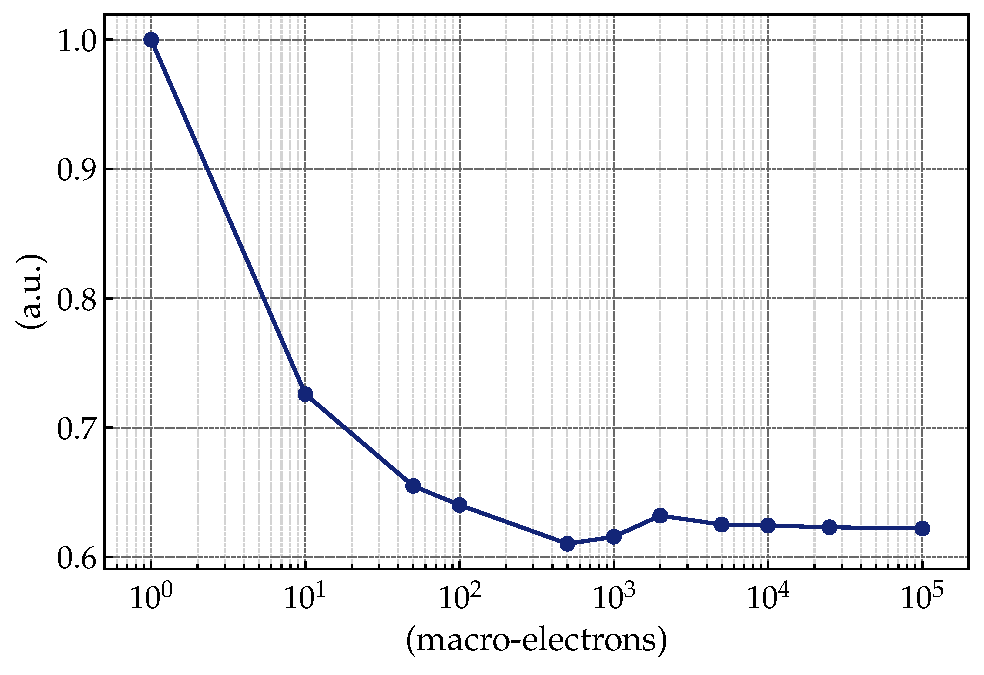
\includegraphics[height=4.5cm]{figures/id18_c01_7p0keV_peak_intensity.pdf}}\\
\end{figure}
\end{document}
